\begin{comment}

Source: https://redmine.upd89.org/redmine/projects/upd89/wiki/API

\end{comment}

\chapter{API}

Die beiden Komponenten \gls{agent} und \gls{controlcenter} kommunizieren über eine API.

\xxx[ Mehr über API allgemein ]
\xxx[ evtl. comments aus JSON entfernen ]
\xxx[ definitiv mehr zum Unterschied hash/full! ]
\xxx[ evtl. table bei A->CC entfernen ]

\begin{figure}
  \centering
    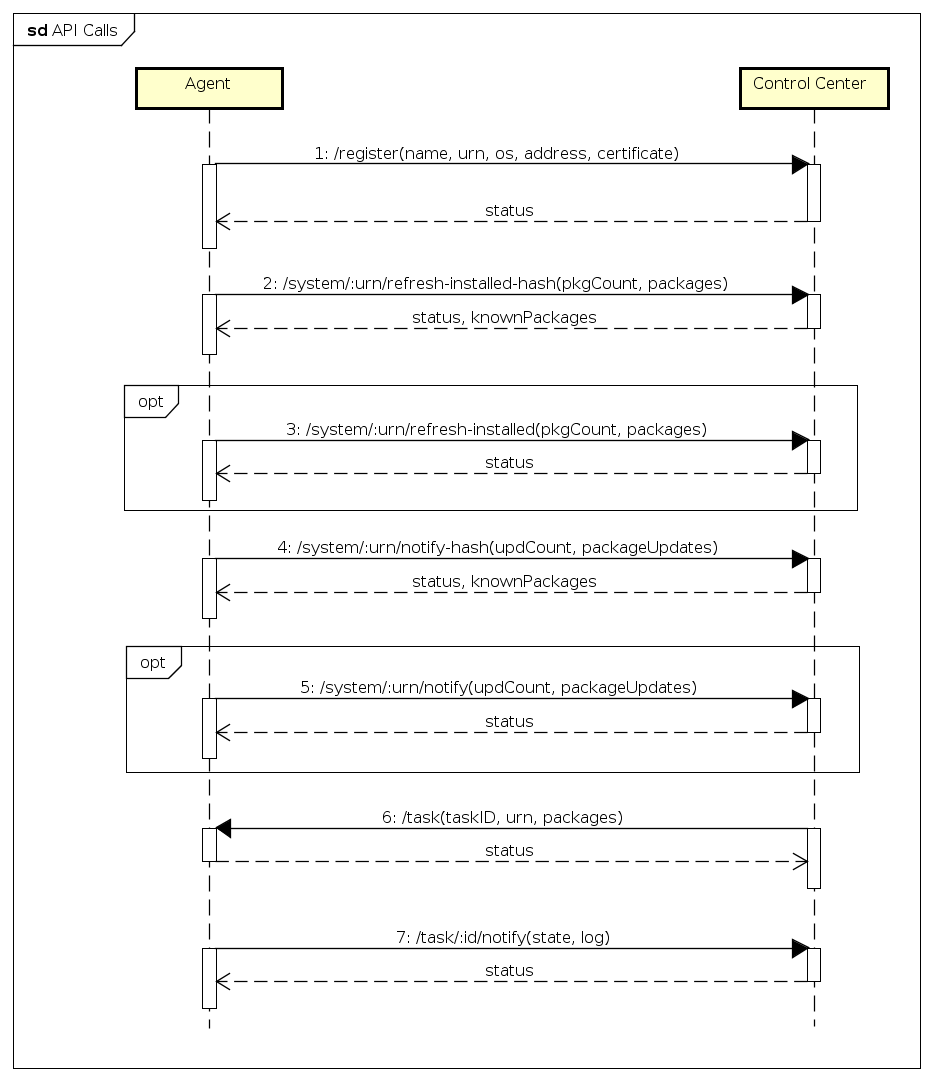
\includegraphics[width=\textwidth]{fig/API_Calls}
  \caption{Sequenzdiagramm bezüglich API-Aufrufe}
  \label{fig:api_sequence_diagram}
\end{figure}

\section*{Status-Codes}

\begin{table}[H]
    \centering
    \caption{Status-Codes}
    \label{api:codes}
    \begin{tabular}{ll}
        \hline
        \textbf{Status} & \textbf{Bedeutung}                                                          \\ \hline
        OK              & Alles war in Ordnung                                                        \\
        ERROR           & Fehler im Ablauf                                                            \\
        infoIncomplete  & Mind. 1 der Hashes ist unbekannt                                            \\
        countMismatch   & System hat eine andere Anzahl installierte Pakete/Updates als gemeldet      \\
        pkgUnknown      & Mindestens eines der gemeldeten Pakete oder Base-Versions ist nicht bekannt \\ \hline
    \end{tabular}
\end{table}


\section*{Control Center}

\begin{table}[H]
    \centering
    \caption{API-Endpunkte auf Seite Control Center}
    \label{api:endpoints_cc}
    \begin{tabular}{ll}
        \hline
        \textbf{Aufruf}                     & \textbf{Details}                                  \\ \hline
        /register                           & A registriert sich beim CC                        \\
        /system/:urn/notify-hash            & A teilt seine anstehenden Updates mit CC via Hash \\
        /system/:urn/notify                 & siehe oben, aber mit vollständigen Informationen  \\
        /system/:urn/refresh-installed-hash & A meldet CC seine installierten Pakete als Hashes \\
        /system/:urn/refresh-installed      & siehe oben, aber mit vollständigen Informationen  \\
        /task/:id/notify                    & A meldet Status zu spezifischem Task              \\ \hline
    \end{tabular}
\end{table}

\subsection*{/register}

\begin{minted}{json}
{
  "name"        : String,
  "urn"         : String,
  "os"          : String,
  "address"     : String,
  "tag"         : String, /*optional*/
  "certificate" : String
}
\end{minted}


Antwort:

\begin{minted}{json}
{
  "status" : "OK"|"ERROR" 
}
\end{minted}

OK: System wurde erfolgreich registriert oder das System existiert bereits. Letzteres kann z.B. bei einer Neuinstallation des Systems vorkommen.
ERROR: Parameter fehlt

\subsection*{/system/:urn/refresh-installed-hash}

\begin{minted}{json}
{
  "pkgCount" : Integer,
  "packages" : [] Array of Strings/Hashes /*can be empty if increment/delta = 0*/
}
\end{minted}

Hinweis: Stimmt der Package-Count mit der Grösse des Package-Arrays überein, dann werden andere (nicht im Array enthaltene aber im CC vermerkte) Pakete auf "Outdated" gesetzt! Wenn das CC bei einem API-Aufruf "countMismatch" liefert, sollte normalerweise dieser Fall eintreten, der Agent sollte also alle installierten Pakete schicken.


Antwort:

\begin{minted}{json}
{
  "status"        : "OK"|"ERROR"|"infoIncomplete"|"countMismatch",
  "knownPackages" : [] Array of Strings/Hashes /*optional unless status === infoIncomplete*/
}
\end{minted}


\subsection*{/system/:urn/refresh-installed}

\begin{minted}{json}
{
  "pkgCount" : Integer,
  "packages" :
  [
    {
      "name"             : String,
      "section"          : String,
      "summary"          : String,
      "homepage"         : String,
      "installedVersion" :
      {
        "version"        : String,
        "sha256"         : String,
        "architecture"   : String,
        "repository"     :
        {
          "archive"      : String,
          "origin"       : String,
          "component"    : String
        }
      },
      "isBaseVersion"    : Boolean,
      "baseVersion"      : /*Optional if isBaseVersion == true*/
      {
        "version"        : String,
        "sha256"         : String,
        "architecture"   : String,
        "repository"     :
        {
          "archive"      : String,
          "origin"       : String,
          "component"    : String
        }
      }
    }
  ]
}
\end{minted}

Hinweis: Stimmt der Package-Count mit der Grösse des Package-Arrays überein, dann werden andere (nicht im Array enthaltene aber im CC vermerkte) Pakete auf 'Outdated' gesetzt! Wenn das CC bei einem API-Aufruf 'countMismatch' liefert, sollte normalerweise dieser Fall eintreten, der Agent sollte also alle installierten Pakete schicken.


Antwort:

\begin{minted}{json}
{
  "status"        : "OK"|"ERROR"|"countMismatch" 
}
\end{minted}

\subsection*{/system/:urn/notify-hash}

\begin{minted}{json}
{
  "name"            : String,  /*optional*/
  "urn"             : String,  /*optional*/
  "os"              : String,  /*optional*/
  "address"         : String,  /*optional*/
  "rebootRequired"  : Boolean, /*optional*/
  "updCount"        : Integer,
  "packageUpdates"  : [] Array of Strings /*can be empty*/
}
\end{minted}

Hinweis: Stimmt der Update-Count mit der Grösse des PackageUpdate-Arrays überein, dann werden andere (nicht im Array enthaltene aber im CC vermerkte) Updates auf "Outdated" gesetzt! Wenn das CC bei einem API-Aufruf "countMismatch" liefert, sollte normalerweise dieser Fall eintreten, der Agent sollte also alle verfügbaren Updates schicken.


Antwort:

\begin{minted}{json}
{
  "status"        : "OK"|"ERROR"|"infoIncomplete"|"countMismatch",
  "knownPackages" : [] Array of Strings /*optional unless status === infoIncomplete*/
}
\end{minted}

\subsection*{/system/:urn/notify}

\begin{minted}{json}
{
  "name"                 : String, /*optional*/
  "urn"                  : String, /*optional*/
  "os"                   : String, /*optional, also covers the PkgVersion's Distribution*/
  "address"              : String, /*optional*/
  "rebootRequired"       : Boolean, /*optional*/
  "updCount"             : Integer,
  "packageUpdates"       : /*can be empty*/
  [
    {
      "name"             : String,
      "candidateVersion" :
      {
        "version"        : String,
        "sha256"         : String,
        "architecture"   : String,
        "repository"     :
        {
          "archive"      : String,
          "origin"       : String,
          "component"    : String
        }
      },
      "baseVersionHash"  : String /*Hash as reference to base version*/
    }
  ]
}
\end{minted}

Hinweis: Stimmt der Update-Count mit der Grösse des PackageUpdate-Arrays überein, dann werden andere (nicht im Array enthaltene aber im CC vermerkte) Updates auf "Outdated" gesetzt! Wenn das CC bei einem API-Aufruf "countMismatch" liefert, sollte normalerweise dieser Fall eintreten, der Agent sollte also alle verfügbaren Updates schicken.


Antwort:

\begin{minted}{json}
{
  "status" : "OK"|"ERROR"|"countMismatch"|"pkgUnknown"
}
\end{minted}

\subsection*{/task/:id/notify}

\begin{minted}{json}
{
  "state" : "Done"|"Failed",
  "log"   : String
}
\end{minted}


Antwort: 

\begin{minted}{json}
{
  "status" : "OK"|"ERROR" 
}
\end{minted}

\section*{Agent}

\begin{table}[H]
    \centering
    \caption{API-Endpunkte auf Seite Agent}
    \label{api:endpoints_a}
    \begin{tabular}{ll}
        \hline
        \textbf{Aufruf}  & \textbf{Details}            \\ \hline
        /task            & A erhält neuen Task von CC  \\ \hline
    \end{tabular}
\end{table}

\subsection*{/task}

\begin{minted}{json}
{
  "taskId"         : Number,
  "urn"            : String,
  "packages"       : 
  [
    {
      "pkgName"    : String,
      "pkgVersion" : String
    }
  ]
}
\end{minted}

Alle Parameter müssen gesetzt sein. Das Paket-Array darf nicht leer sein.


Antwort:

\begin{minted}{json}
{
  "status" : "OK"|"ERROR" 
}
\end{minted}